\documentclass[10pt]{beamer}


\usepackage{introLatex}
\usepackage{shortcutLatex}



% Thème utilisé ici 
\usetheme{default}

% Pour les images
\usepackage{graphicx}

% Dossier où se trouvent les images
\graphicspath{{imagesdiapo/}}

% Pour la police des expressions mathématiques ou du texte
%\usefonttheme[onlymath]{serif}
\usefonttheme{serif}

\usepackage{ragged2e}
%\usepackage{algorithmicx}
\usepackage{algorithm}
%\usepackage{algorithmic}
\usepackage{algpseudocode}


\setbeamertemplate{title page}{%
\centering
\color{cyan}
\vspace*{8pt}

\includegraphics[scale=0.05]{Logo_ENSTA.png}
\hspace*{80pt}

\includegraphics[scale=0.20]{logo_uma.png}
\hfill

\includegraphics[scale=0.15]{parisSaclay.jpg}\\
\vspace*{10pt}
\large \textbf{\inserttitle} \\
\vspace*{6pt}
\normalsize \insertsubtitle \\
\vspace*{10pt}
\color{black}
\rule{2cm}{0.5pt}\\
\vspace{10pt}
\normalsize \insertauthor\\
\vspace*{10pt}
\small \textit{\insertinstitute}\\

\vspace{12pt}
\color{cyan}
\insertdate\\
\color{black}
}


\setbeamertemplate{navigation symbols}{}


% Page de garde
\title[Parallélisation d'une méthode d'éléments finis]{Parallélisation d'une méthode d'éléments finis pour la résolution de l'équation de la chaleur}
\subtitle{Calcul parallèle scientifique - Soutenance de Projet\\
Master 2 Analyse Modélisation Simulation}
\author{Pierre-Emmanuel Emeriau \& Gaétan Facchinetti}
\institute{Université Paris-Saclay \\ Ecole Nationale Supérieure des Techniques Avancées \\ Ecole Normale Supérieure Paris-Saclay}
\date{24 novembre 2016}


\setbeamertemplate{section in toc}{\inserttocsectionnumber.~\inserttocsection}


\newcommand{\footHeadLine}{%
\logo{\pgfputat{\pgfxy(-1.0,1.2)}{\pgfbox[center,base]{
\includegraphics[scale=0.1]{parisSaclay.jpg}}}}
\setbeamertemplate{footline}{%
\raggedright%
\vspace*{-12pt}%
\color{white}%
\hspace*{2em}%
{\sffamily\small\color{white} Emeriau - Facchinetti \hspace*{4pt}/ \hspace*{4pt} 16 novembre 2016 \hfill \color{black}\thepage\hspace*{2em}}%
\vspace*{2pt}%
}%
%
\setbeamertemplate{headline}{%
\ifnum \thesubsection>0%
\vspace*{6pt}%
\raggedright%
\hspace*{5em}%
{\sffamily\normalsize\bfseries\color{white}\thesection.~\insertsection\\}%
\vspace*{3pt}
\hspace*{9em}
{\sffamily\small\bfseries\color{white}\thesubsection.~\insertsubsection}%
\hspace*{2em}%
\else 
\vspace*{10pt}%
\raggedright%
\hspace*{5em}%
{\sffamily\normalsize\bfseries\color{white}\thesection.~\insertsection\\}%
\vspace*{3pt}
\fi%
}
}

\newcommand{\sommaire}{%
\setbeamertemplate{footline}{}
\setbeamertemplate{headline}{}
\logo{}
\begin{frame}
	\vspace*{22pt}
	\tableofcontents[currentsection]
\end{frame}
\footHeadLine{}
}

% On declare les images utilisee en logo et en fond
\pgfdeclareimage[height=96mm,width=128mm]{fond}{Presentation3.pdf}

% On definit le fond
\setbeamertemplate{background}{\pgfuseimage{fond}}






\begin{document}

	\begin{frame}[t]
	\titlepage
	\end{frame}


	\begin{frame}
	\vspace*{22pt}
	\tableofcontents
	\end{frame}





\footHeadLine{}

\section{Introduction du problème}
\subsection{L'équation de la chaleur}

\sommaire{}

	\begin{frame}
		\justifying
		\vspace*{22pt}
		On considère un domaine $\Omega$ de $\R^{2}$.\\
		Nous ne nous interessons qu'au problème \textit{stationnaire}. \\

		\begin{itemize}
		\item $u(\xv)$ la température au point $\xv\in\Omega$. \\
 		\item $\jv(\xv)$ le flux de chaleur au point $\xv\in\Omega$.\\
 		\item $f(\xv)$ Energie produite par unité de surface au point $\xv\in\Omega$. \\
 		\item $\lambda$ conductivité termique, constante pour un matériaux uniforme.\\
 		
		\end{itemize}
		\vspace*{11pt}

		
		La conservation de l'energie et la loi de Fourier donnnent alors :\\
		\begin{equation}
		%\frac{\partial u}{\partial t} + 
		\text{div}(\jv) = f \quad \text{et} \quad \jv = - \lambda\nablav u
		\end{equation}

		\vspace*{11pt}
		D'où, l'équation de la chaleur en régme stationnaire : \\
		\begin{equation}
		\begin{cases}
		\Delta u  = f  & \text{ dans } \Omega \\
		u  =  g  & \text{ sur } \partial\Omega
		\end{cases}
		\label{eq:pb}
		\end{equation}
	\end{frame}



\subsection{La métode des éléments finis}

	\begin{frame}
	
		\vspace*{33pt}
		On considère un relèvement $u_0$ de $g \in H^{1/2}(\Omega)$ dans $H^{1}(\Omega)$. \\
		On pose $\tilde{u} = u-u_0$. Le problème (2) se réécrit : \\
		\vspace*{11pt}
		Trouver $\tilde{u} \in H^{1}_{0}(\Omega)$ tel que
		\begin{equation}
		\forall v \in H^{1}_{0} \quad \int_{\Omega}{\nabla \tilde{u}}{\nabla v} = \int_{\Omega}{fv}
		\end{equation}

		On effectue une résolution par éléments finis de Lagrange $P_1$.\\
		Soit $T = \{\tau_l\}_l$ une famille de triangulation de $\Omega$.\\
		Soit $V_h^{0} = \{v \in \Cc^{0}(\Omega) \text{ | } \forall l \quad v_{|\tau_l} \in P_1(\tau_l) \}$.\\
		Soit $(\phi_j)_{1 \le j \le N_i}$ une base de $V_h^{0}$ avec $N_i=dim(V_h^{0})$.  \\
		\vspace*{11pt}
		On décompose $\tilde{u}$ sur cette base :  $\tilde{u} = \sum_{j=1}^{N_i}{\tilde{u}_j\phi_j}$. \\

		\begin{equation}
		\text{Ainsi,} \quad (3) \Rightarrow \forall k \in \bbrac{1,N_i} \quad \sum_{j=1}^{N_i}{\tilde{u}_j\int_{\Omega}{\nabla \phi_j \nabla \phi_k}} = \int_{\Omega}{f\phi_k}
		\end{equation}

	\end{frame}



	\begin{frame}

		\justifying
		\vspace*{22pt}
		Ceci permettrait de réécrire le problème sous forme matricielle : \\
		\vspace*{11pt}
		On pose $\forall (p,q) \in \bbrac{1,N_i} \quad \tilde{\K}_{p,q} = \int_{\Omega}{\nabla \phi_p \nabla \phi_q}$. \\
		Ainsi que $\forall p \in \bbrac{1,N_i} \quad \tilde{f}_p = \int_{\Omega}{f\phi_p}$. \\
		On écrit $\tilde{\uv} = {(\tilde{u}_1, \dots, \tilde{u}_N)}^{T}$.

		\begin{equation}
			\tilde{\K} \uv = \tilde{\fv}
		\end{equation}

		\vspace*{11pt}
		Prise en compte dans le code (lors de l'assemblage et de la pseudo-élimination) du fait que l'on résout sur $u$ et non $\tilde{u}$. En notant $u_p$ la valeur de $u$ au noeud $p$ et le vecteur $\uv = {(u_1, \dots, u_N)}^{T}$ avec $N$ le nombre total de points ($N = N_i + N_b$ avec $N_b$ le nombre de points sur le bord) le système s'écrit alors : 

		\begin{equation}
			\K_{elim} \uv = \fv_{elim}
		\end{equation}



	\end{frame}




\section{Méthode de travail}
\sommaire{}

\subsection{Découpage du problème sur les processeurs}


	\begin{frame}	
		\vspace*{33pt}
		Définition des variables de parallélisation
		\begin{itemize}
			\item myRank : le rank du processeur sur lequel on travaille
			\item nbTask : le nombre de tâches égal au nombre de partitions + 1
		\end{itemize}
		C'est le processeur 0 qui s'occupe de l'interface\\
		\vspace*{11pt}

		Organisation du découpage : \\
		\begin{figure}[H]
		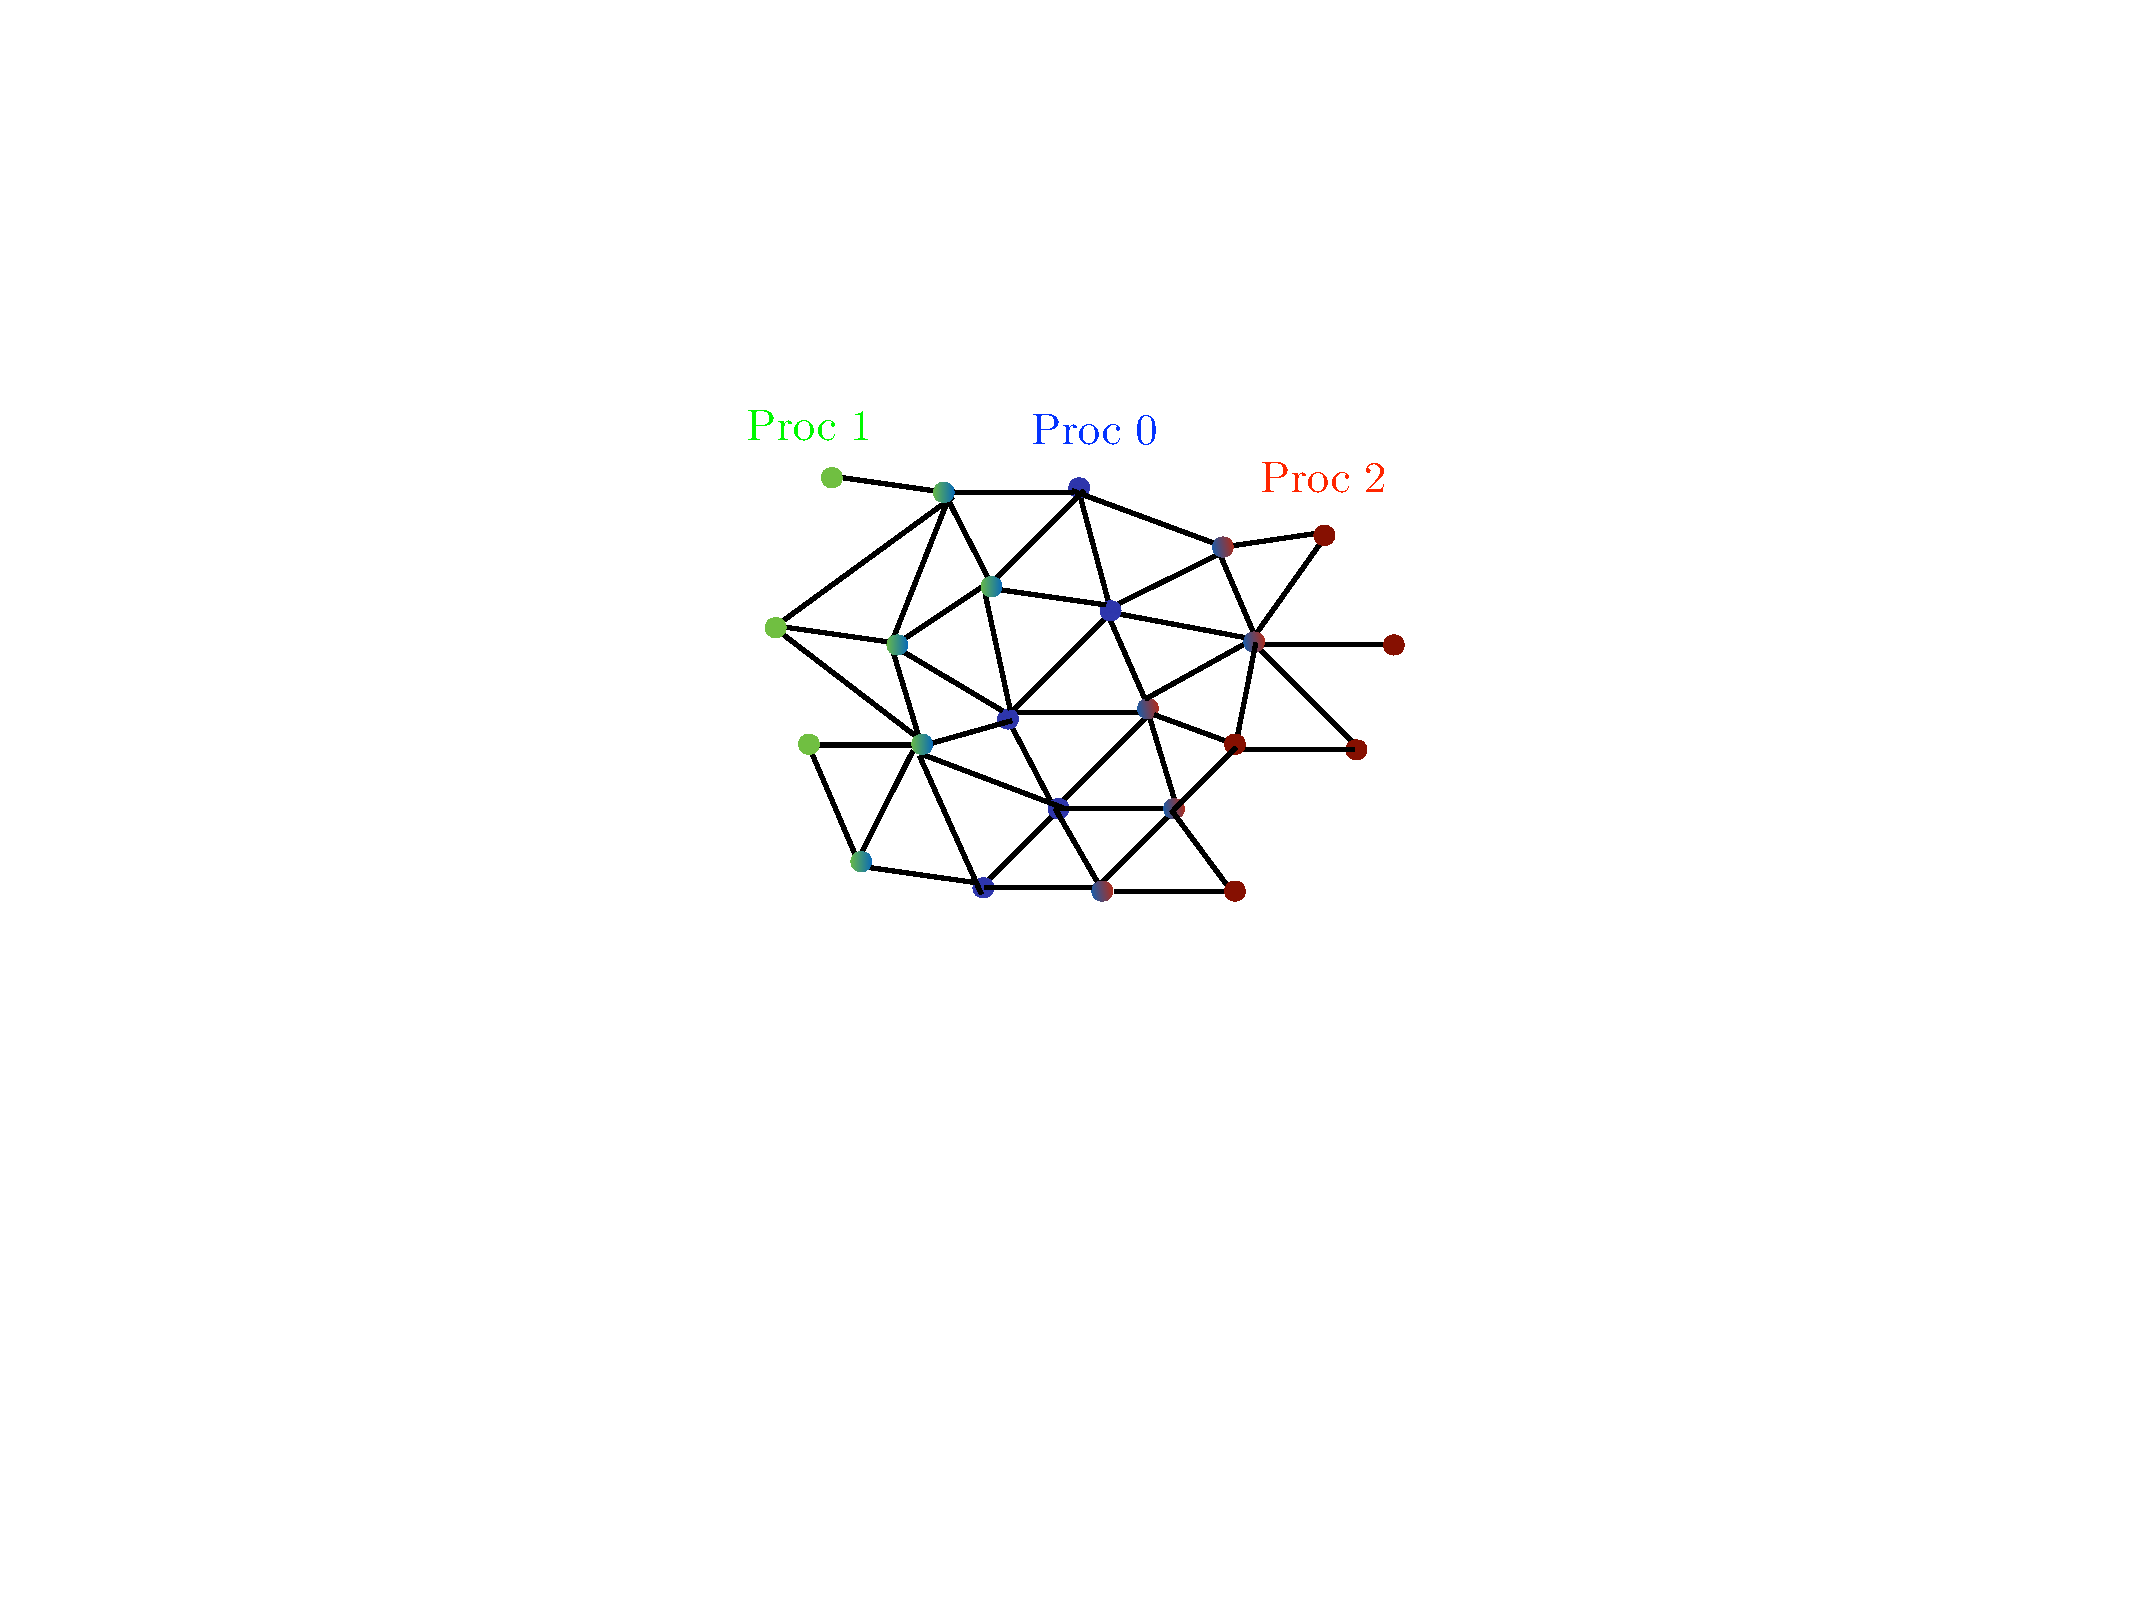
\includegraphics[scale=0.4]{Essai.pdf}
		\caption{Schéma du découpage entre processeurs}
		\end{figure}


	

	\end{frame}



	\subsection{Le découpage en pratique}

	\begin{frame}

		\vspace*{22pt}
		Definition des vecteurs et matrices sur chaque processeur : 
		\begin{itemize}
			\item Définition des vecteurs de taille globale $N$
			\item Définition des matrices \textit{sparse} de taille globale $N$
		\end{itemize}

		\vspace{11pt}

		Problèmes qu'il nous a fallu résoudre au préalable : 

		\begin{itemize}
			\item Construction de tableau étiquetant les noeurs sur chqaue proc
			\item Attribution à chaque processeur de ses triangles et noeuds
			\item Initialisation/communication des listes de noeuds à communiquer
			\item Pseudo-elimination sur l'ensemble des noeuds du bord
			\item Nettoyage des lignes incompètes de $\K_{elim}$ 
			\item Suppression des coefficients parasites de $\fv_{elim}$

		\end{itemize}
	\end{frame}		





\section{Parallélisation des solveurs}
\sommaire{}

\subsection{Méthode de Jacobi}

	\begin{frame}	

	\vspace*{22pt}
	Algorithme avec communications : 
	\vspace*{-10pt}
		\begin{algorithm}[H]
			\begin{algorithmic}[1]
				\State $M = diag(\K_{elim})$ et $N = - \K_{elim} + M$
				\For{$k=1,1000$}
				\State $\uv_k = M^{-1}N\uv_k + M^{-1}\fv_{elim}$
				\State \Call{\color{blue}MPI\_BCAST\color{black}}{$p_0 \rightarrow p_{\text{myRank}\neq 0}$, $\uv_{k|\text{interface}}$}
					\If{myRank $== 0$}
						\For{$i = 1,\text{nbTask-1}$}
							\State \Call{\color{blue}MPI\_RECV\color{black}}{$p_i \rightarrow p_0$, $\uv_{k|\text{voisins interface}}$}
						\EndFor
					\Else
						\State \Call{\color{blue}MPI\_SEND\color{black}}{$ p_{\text{myRank}} \rightarrow p_0 $, $\uv_{k|\text{voisins interface}}$}
					\EndIf
					\State \color{red}Calcul de la norme du residu : $\|\rv_k\|$\color{black}
				\EndFor
				\Statex
				\State \color{red} Reconstruction de la solution sur $p_0$ \color{black}
			\end{algorithmic}
		\end{algorithm}
		


	\end{frame}	




	\begin{frame}	

	\vspace*{22pt}
	Calcul de la norme du résidu : 


	\begin{algorithm}[H]
		\begin{algorithmic}[1]
			\State ...
			\State $\rv_k = \K_{elim}\uv_k - \fv_{elim}$
			\State $S = (\rv_k, \rv_k)$
			\State \Call{\color{blue}MPI\_ALLREDUCE\color{black}}{$ p_{\text{myRank}} \rightarrow p_0$, MPI\_SUM, $S$, Res : $S_t$}
			\State $\|\rv_k\| = \sqrt{S_t}$
			\If{$\|\rv_k\| < \epsilon \|\rv_0\|$}
				\State EXIT
			\EndIf
			\State ...
		\end{algorithmic}
	\end{algorithm}

	Reconstruction de la solution : 


	\begin{algorithm}[H]
		\begin{algorithmic}[1]
			\State ...
			\State \Call{\color{blue}MPI\_REDUCE\color{black}}{$ p_{\text{myRank}} \rightarrow p_0$, MPI\_SUM, $\uv_{k|\text{myRank}}$, Res : $\uv$}
		\end{algorithmic}
	\end{algorithm}
		

	\end{frame}	




\subsection{Méthode de Gauss-Seidel}

	\begin{frame}	
		Frame de test
	\end{frame}	



\section{Resultats}

	\begin{frame}
		Visualisation de la solution du ParaView

	\end{frame}

	\begin{frame}
		Comparaison des temps de calcul sur gin : 

	\end{frame}




\end{document}